%----------------------------------------------------------------------------------------
%	PACKAGES AND OTHER DOCUMENT CONFIGURATIONS
%----------------------------------------------------------------------------------------

\documentclass{article}

\usepackage{fancyhdr} % Required for custom headers
\usepackage{lastpage} % Required to determine the last page for the footer
\usepackage{extramarks} % Required for headers and footers
\usepackage{graphicx} % Required to insert images
\usepackage{amsmath, amssymb} % Required for Maths
\usepackage{mathtools} % Required for Maths
\usepackage{enumerate}
\usepackage{mathtools}
\usepackage{textcomp}
\usepackage{gensymb}
\usepackage{siunitx}
\usepackage{empheq}
\usepackage{ulem}
\usepackage{amssymb}

% Margins
\topmargin=-0.45in
\evensidemargin=0in
\oddsidemargin=0in
\textwidth=6.5in
\textheight=9.0in
\headsep=0.25in 

\linespread{1.1} % Line spacing

% Set up the header and footer
\pagestyle{fancy}
\lhead{\hmwkAuthorName} % Top left header
\chead{\hmwkClass\ (\hmwkClassInstructor\ \hmwkClassTime): \hmwkTitle} % Top center header
\rhead{\firstxmark} % Top right header
\lfoot{\lastxmark} % Bottom left footer
\cfoot{} % Bottom center footer
\rfoot{Page\ \thepage\ of\ \pageref{LastPage}} % Bottom right footer
\renewcommand\headrulewidth{0.4pt} % Size of the header rule
\renewcommand\footrulewidth{0.4pt} % Size of the footer rule

\setlength\parindent{0pt} % Removes all indentation from paragraphs

%----------------------------------------------------------------------------------------
%	DOCUMENT STRUCTURE COMMANDS
%	Skip this unless you know what you're doing
%----------------------------------------------------------------------------------------

% Header and footer for when a page split occurs within a problem environment
\newcommand{\enterProblemHeader}[1]{
\nobreak\extramarks{#1}{#1 continued on next page\ldots}\nobreak
\nobreak\extramarks{#1 (continued)}{#1 continued on next page\ldots}\nobreak
}

% Header and footer for when a page split occurs between problem environments
\newcommand{\exitProblemHeader}[1]{
\nobreak\extramarks{#1 (continued)}{#1 continued on next page\ldots}\nobreak
\nobreak\extramarks{#1}{}\nobreak
}

\setcounter{secnumdepth}{0} % Removes default section numbers
\newcounter{homeworkProblemCounter} % Creates a counter to keep track of the number of problems

\newcommand{\homeworkProblemName}{}
\newenvironment{homeworkProblem}[1][Problem \arabic{homeworkProblemCounter}]{ % Makes a new environment called homeworkProblem which takes 1 argument (custom name) but the default is "Problem #"
\stepcounter{homeworkProblemCounter} % Increase counter for number of problems
\renewcommand{\homeworkProblemName}{#1} % Assign \homeworkProblemName the name of the problem
\section{\homeworkProblemName} % Make a section in the document with the custom problem count
\enterProblemHeader{\homeworkProblemName} % Header and footer within the environment
}{
\exitProblemHeader{\homeworkProblemName} % Header and footer after the environment
}

\newcommand{\problemAnswer}[1]{ % Defines the problem answer command with the content as the only argument
\noindent\framebox[\columnwidth][c]{\begin{minipage}{0.98\columnwidth}#1\end{minipage}} % Makes the box around the problem answer and puts the content inside
}

\newcommand{\homeworkSectionName}{}
\newenvironment{homeworkSection}[1]{ % New environment for sections within homework problems, takes 1 argument - the name of the section
\renewcommand{\homeworkSectionName}{#1} % Assign \homeworkSectionName to the name of the section from the environment argument
\subsection{\homeworkSectionName} % Make a subsection with the custom name of the subsection
\enterProblemHeader{\homeworkProblemName\ [\homeworkSectionName]} % Header and footer within the environment
}{
\enterProblemHeader{\homeworkProblemName} % Header and footer after the environment
}

%----------------------------------------------------------------------------------------
%	NAME AND CLASS SECTION
%----------------------------------------------------------------------------------------

\newcommand{\hmwkTitle}{Homework\ \#2} % Assignment title
\newcommand{\hmwkDueDate}{Wednesday,\ October\ 7,\ 2015} % Due date
\newcommand{\hmwkClass}{ENPM 808M} % Course/class
\newcommand{\hmwkClassTime}{4:00 PM} % Class/lecture time
\newcommand{\hmwkClassInstructor}{Dr. William Levine} % Teacher/lecturer
\newcommand{\hmwkAuthorName}{Kanishka Ganguly} % Your name

%----------------------------------------------------------------------------------------
%	TITLE PAGE
%----------------------------------------------------------------------------------------

\title{
\vspace{2in}
\textmd{\textbf{\hmwkClass:\ \hmwkTitle}}\\
\normalsize\vspace{0.1in}\small{Due\ on\ \hmwkDueDate}\\
\vspace{0.1in}\large{\textit{\hmwkClassInstructor\ \hmwkClassTime}}
\vspace{3in}
}

\author{\textbf{\hmwkAuthorName}}
\date{} % Insert date here if you want it to appear below your name

%----------------------------------------------------------------------------------------

\begin{document}

\maketitle

%----------------------------------------------------------------------------------------
%	TABLE OF CONTENTS
%----------------------------------------------------------------------------------------

%\setcounter{tocdepth}{1} % Uncomment this line if you don't want subsections listed in the ToC

\newpage
\tableofcontents
\newpage

%----------------------------------------------------------------------------------------
%	PROBLEM 1
%----------------------------------------------------------------------------------------
\begin{homeworkProblem}
Given $A$ is a rotation matrix. So, $A \in SO(2)$, or the \textbf{special orthogonal group} of dimension 2 whose determinant is $1$ or $-1$. Here the $2$ in $SO(2)$ denotes that $A$ belongs to the $2-D$ rotation group.\\
Let 
\[
A = 
\begin{bmatrix}
a & b\\
c & d
\end{bmatrix}
\]\\
We know (from identity) that since $A \in SO(2)$, $A \in SO(3) \ \text{also}$. Using this identity and Cramer's Rule, we have
\[
A^{-1} = 
\begin{bmatrix}
d & -b\\
-c & a
\end{bmatrix}
=
\begin{bmatrix}
a & c\\
b & d
\end{bmatrix}
\]\\
This implies that $a = d$ and $b = -c$. Thus we have
\[
A = 
\begin{bmatrix}
a & -c\\
c & a
\end{bmatrix}
\]\\

Since it is given that $det(A) = 1$, we have $a^2 + c^2 = 1$.\\\\
Let us define $\theta = tan^{-1}(\frac{c}{a})$. This gives us
\begin{align}
cos(\theta) = a\\
sin(\theta) = c
\end{align}

Thus, there exists a unique $\theta$ such that $A$ is of the form
\[
A = 
\begin{bmatrix}
cos(\theta) & -sin(\theta)\\
sin(\theta) & cos(\theta)
\end{bmatrix}
\]\\
\end{homeworkProblem}

%----------------------------------------------------------------------------------------
%	PROBLEM 2
%----------------------------------------------------------------------------------------

\begin{homeworkProblem} % Custom section title
Let us consider the following sequence of rotations:
\begin{enumerate}
\item Rotate by $\phi$ about world $x$-axis. Let this be represented by $R_{x,\phi}$.
\item Rotate by $\theta$ about current $z$-axis. Let this be represented by $R_{z,\theta}$.
\item Rotate by $\psi$ about current $x$-axis. Let this be represented by $R_{x,\psi}$.
\item Rotate by $\alpha$ about world $z$-axis. Let this be represented by $R_{z,\alpha}$.
\end{enumerate}
By convention, we apply the rotations in the following order:
\begin{enumerate}
\item Apply all the rotations in the world coordinate axis in the \textbf{last in, first out} order.
\item Apply all the rotations in the current coordinate axis in the \textbf{first in, first out} order.
\end{enumerate}
So, we have 
\begin{align}
R_{final} = R_{z,\alpha} \times R_{x,\phi} \times R_{z,\theta} \times R_{x,\psi}
\end{align}
\end{homeworkProblem}

%----------------------------------------------------------------------------------------
%	PROBLEM 3
%----------------------------------------------------------------------------------------

\begin{homeworkProblem}
The Euler angles are given as $(\phi, \theta,\psi) \equiv (\frac{\pi}{2}, 0, \frac{\pi}{4})$
We have the general rotation matrix $A$ given by
\[
A=
\begin{bmatrix}
 a_{11} & a_{12} & a_{13}\\
 a_{21} & a_{22} & a_{23}\\
 a_{31} & a_{32} & a_{33}
\end{bmatrix}
\]
Also, we have the following component matrices:
\begin{align}
%--- Matrix D ---%
\begin{rcases}
D \equiv
\begin{bmatrix}
cos(\phi) & sin(\phi) & 0\\
-sin(\phi) & cos(\phi) & 0\\ 
0 & 0 & 1
\end{bmatrix}
\end{rcases} \phi \ \text{about z-axis}\\
%--- Matrix C ---%
\begin{rcases}
C \equiv
\begin{bmatrix}
1 & 0 & 0\\
0 & cos(\theta) & sin(\theta)\\
0 & -sin(\theta) & cos(\theta)
\end{bmatrix}
\end{rcases} \theta \ \text{about former x-axis}\\
%--- Matrix B ---%
\begin{rcases}
B \equiv
\begin{bmatrix}
cos(\psi) & sin(\psi) & 0\\
-sin(\psi) & cos(\psi) & 0\\
0 & 0 & 1
\end{bmatrix}
\end{rcases} \psi \ \text{about former z-axis}
\end{align}

This gives us the following:
\begin{align}
a_{11} = cos(\psi)cos(\phi)-cos(\theta)sin(\phi)sin(\psi) = -\frac{1}{\sqrt{2}}\\
a_{12} = cos(\psi)sin(\phi)+cos(\theta)cos(\phi)sin(\psi) = -\frac{1}{\sqrt{2}}\\
a_{13} = sin(\psi)sin(\theta) = 0\\
a_{21} = -sin(\psi)cos(\phi)-cos(\theta)sin(\phi)cos(\psi) = \frac{1}{\sqrt{2}}\\
a_{22} = -sin(\psi)sin(\phi)+cos(\theta)cos(\phi)cos(\psi) = -\frac{1}{\sqrt{2}}\\
a_{23} = cos(\psi)sin(\theta) = 0\\
a_{31} = sin(\theta)sin(\phi) = 0\\
a_{32} = -sin(\theta)cos(\phi) = 0\\
a_{33} = cos(\theta) = 1
\end{align}
Thus we get
\[
R^0_1 = 
\begin{bmatrix}
-\frac{1}{\sqrt{2}} & -\frac{1}{\sqrt{2}} & 0\\
\frac{1}{\sqrt{2}} & -\frac{1}{\sqrt{2}} & 0\\
0 & 0 & 1
\end{bmatrix}
\]

The direction of the $x_1$ axis relative to the base frame is given by the first column of $R^0_1$ as \Big( $-\frac{1}{\sqrt{2}}, \frac{1}{\sqrt{2}}, 0$\Big)
\end{homeworkProblem}
\clearpage

%----------------------------------------------------------------------------------------
%	PROBLEM 4
%----------------------------------------------------------------------------------------

\begin{homeworkProblem}
It is given that
\begin{align}
H = Rot_{x,\alpha}Trans_{x,b}Trans_{z,d}Rot_{z,\theta}
\end{align}
\begin{enumerate}[I. ]
\item 
Consider the first pair of transformation $Rot_{x,\alpha}Trans_{x,b}$.\\
Here, by rotating by $\alpha$ around the $x$-axis, i.e. $Rot_{x,\alpha}$, we have a change in the $y$ and $z$ axes only, while the $x$-axis is preserved. Or, $(x, y, z) \to (x, y', z')$.\\
Now, with the translation $Trans_{x,b}$, which is the translation along the $x$-axis by a distance $b$, we have $(x, y, z) \to (x+b, y, z)$. Thus, \uuline{all axes are preserved in translation.}\\

\item 
So, by similar logic, we have $Trans_{z,d}Rot_{z,\theta}$ giving the same result, i.e. \uuline{translation and rotation about the same axis is commutative, since the orientation of the axis is preserved.}\\

\item 
Moving on to $Rot_{x,\alpha}Rot_{z,\theta}$, since the rotations are first $\alpha$ around $x$-axis and then $\theta$ around $z$-axis, we have $y, z$ axes being affected in the former and $x, y$ axes being affected in the latter. In such a case, the order of transformation matters. Thus, $Rot_{x,\alpha}$ and $Rot_{z,\theta}$ are \uuline{not commutative since they are transformations on two different axes.}

\item
Taking $Rot_{x,\alpha}$ and $Trans_{z,d}$, we have the case of rotation and translation on different axes, where $Rot_{x,\alpha}$ is along the $x$-axis which affects the $y,z$ orientation while $Trans_{z,d}$ is along the $z$-axis which affects the $z$ orientation. Thus, in this case also, the order in which the transformations are applied matter since they are applied on different axes. So, \uuline{rotation and translation along different axes are not commutative, since orientation of axes are not preserved.}

\item
The same logic applies to the case of $Trans_{x,b}$ and $Rot_{z,\theta}$, where the $x$-axis is affected by the former transformation and the $y,z$ axes are affected by the latter.
\end{enumerate}

Thus, we have the following conclusions:
\begin{align}
Rot_{x,\alpha}Trans_{x,b} = Trans_{x,b}Rot_{x,\alpha}\\
Trans_{z,d}Rot_{z,\theta} = Rot_{z,\theta}Trans_{z,d}\\
Trans_{x,b}Trans_{z,d} = Trans_{z,d}Trans_{x,b}\\
Rot_{x,\alpha}Rot_{z,\theta} \neq Rot_{z,\theta}Rot_{x,\alpha}\\
Rot_{x,\alpha}Trans_{z,d} \neq Trans_{z,d}Rot_{x,\alpha}\\
Trans_{x,b}Rot_{z,\theta} \neq Rot_{z,\theta}Trans_{x,b}
\end{align}

From this, we have the following possible permutations of $H = Rot_{x,\alpha}Trans_{x,b}Trans_{z,d}Rot_{z,\theta}$:
\begin{align}
H = Rot_{x,\alpha}Trans_{z,d}Trans_{x,b}Rot_{z,\theta}\\
H = Trans_{x,b}Rot_{x,\alpha}Trans_{z,d}Rot_{z,\theta}\\
H = Trans_{x,b}Rot_{x,\alpha}Rot_{z,\theta}Trans_{z,d}\\
H = Rot_{x,\alpha}Trans_{x,b}Rot_{z,\theta}Trans_{z,d}
\end{align}
\end{homeworkProblem}
\clearpage

%----------------------------------------------------------------------------------------
%	PROBLEM 5
%----------------------------------------------------------------------------------------

\begin{homeworkProblem}
\problemAnswer{ % Answer
\begin{center}
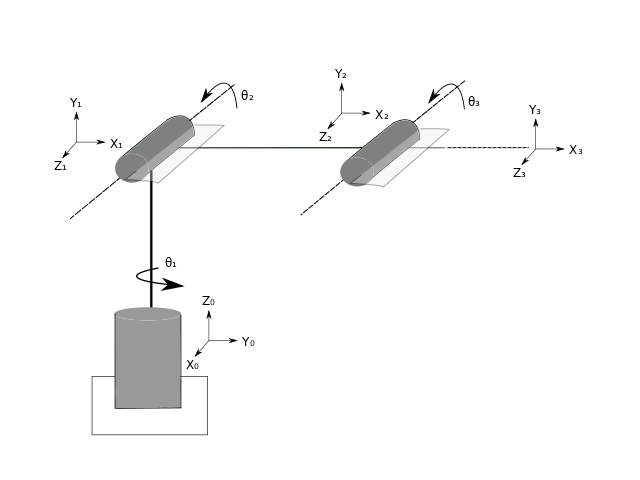
\includegraphics[width=0.75\columnwidth]{img/3-6.png} % Q5_1st Image
\end{center}
}
\vspace{20pt}
Three-link Articulated Robot

We have, for each link $i$ in the robot, the following homogenous transformation
\begin{align}
A_i = R_{z,\theta_i}Trans_{z,d_i}Trans_{x,a_i}R_{x,\alpha_i}\\
A_i=
\begin{bmatrix}
c_{\theta_i} & -s_{\theta_i}c_{\alpha_i} & s_{\theta_i}s_{\alpha_i} & a_ic_{\theta_i}\\
s_{\theta_i} & c_{\theta_i}c_{\alpha_i} & -c_{\theta_i}s_{\alpha_i} & a_is_{\theta_i}\\
0 & s_{\alpha_i} & c_{\alpha_i} & d_i\\
0 & 0 & 0 & 1
\end{bmatrix}
\end{align}
\\
Thus, we have the following table for each of the links:\\
\begin{center}
\begin{tabular}{|l|l|l|l|l|{c}r}
\hline
Link ($i$) & $a_i$ & $\alpha_i$ & $d_i$ & $\theta_i$\\
\hline
1 & $0$ & $90$ & $0$ & $\theta_1$\\
2 & $a_2$ & $0$ & $0$ & $\theta_2$\\
3 & $a_3$ & $0$ & $0$ & $\theta_3$\\
\hline
\end{tabular}
\end{center}

So, we have three homogenous matrices for each of the three links as follows:
\begin{align}
A_1=
\begin{bmatrix}
c_{\theta_1} & 0 & s_{\theta_1} & 0\\
s_{\theta_1} & 0 & -c_{\theta_1} & 0\\
0 & 1 & 0 & 0\\
0 & 0 & 0 & 1
\end{bmatrix}\\
A_2=
\begin{bmatrix}
c_{\theta_2} & -s_{\theta_2} & 0 & a_2c_{\theta_2}\\
s_{\theta_2} & c_{\theta_2} & 0 & a_2s_{\theta_2}\\
0 & 0 & 1 & 0\\
0 & 0 & 0 & 1
\end{bmatrix}\\
A_3=
\begin{bmatrix}
c_{\theta_3} & -s_{\theta_3} & 0 & a_3c_{\theta_3}\\
s_{\theta_3} & c_{\theta_3} & 0 & a_3s_{\theta_3}\\
0 & 0 & 1 & 0\\
0 & 0 & 0 & 1
\end{bmatrix}
\end{align}
Combining the three, we get:
\begin{align}
T^0_3 = A_1 \times A_2 \times A_3 = 
\begin{bmatrix}
r_{11} & r_{12} & r_{13} & d_x\\
r_{21} & r_{22} & r_{23} & d_y\\
r_{31} & r_{32} & r_{33} & d_z\\
0 & 0 & 0 & 1
\end{bmatrix}
\end{align}
where
\begin{align}
r_{11} = c_1c_2c_3 - c_1s_2s_3 = c_1c_{23}\\
r_{12} = -c_1c_2c_3 - c_1s_3c_2 = -c_1s_{23}\\
r_{13} = s_1\\
d_x = a_2c_1c_2 + a_3c_1c_2c_3 - a_3c_1s_2s_3 = a_2c_1c_2 + a_3c_1c_{23}\\
r_{21} = c_2c_3s_1 - s_1s_2s_3 = s_2c_{23}\\
r_{22} = -c_2s_1s_3 - c_3s_1s_2 = -s_1s_23\\
r_{23} = -c_1\\
d_y = a_2c_2s_1 + a_3c_2c_3s_1 -a_3s_1s_2s_3 = a_2c_2s_1 + a_3s_1c_{23}\\
r_{31} = c_2s_3 + c_3s_2 = s_23\\
r_{32} = c_2c_3 - s_2s_3 = c_{23}\\
r_{33} = 0\\
d_z = a_2s_2 + a_3c_2s_3 + a_3c_3s_2 = a_2s_2 + a_3s_{23}
\end{align}
\end{homeworkProblem}
\clearpage

%----------------------------------------------------------------------------------------
%	PROBLEM 6
%----------------------------------------------------------------------------------------

\begin{homeworkProblem}
The six-link chain can be broken up into two types of chains, namely an elbow manipulator and a spherical wrist.\\
Thus, we have
\begin{center}
\begin{tabular}{|l|l|l|l|l|{c}r}
\hline
Link ($i$) & $a_i$ & $\alpha_i$ & $d_i$ & $\theta_i$\\
\hline
1 & $0$ & $90$ & $0$ & $\theta_1$\\
2 & $a_2$ & $0$ & $0$ & $\theta_2$\\
3 & $a_3$ & $0$ & $0$ & $\theta_3$\\
4 & $0$ & $-90$ & $0$ & $\theta_4$\\
5 & $0$ & $90$ & $0$ & $\theta_5$\\
6 & $0$ & $0$ & $d_6$ & $\theta_6$\\
\hline
\end{tabular}
\end{center}
The 6 homogenous matrices for each of the links are as follows:
\begin{align}
A_1 = 
\begin{bmatrix}
c_{\theta_1} & 0 & s_{\theta_1} & 0\\
s_{\theta_1} & 0 & -c_{\theta_1} & 0\\
0 & 1 & 0 & 0\\
0 & 0 & 0 & 1
\end{bmatrix}\\
A_2=
\begin{bmatrix}
c_{\theta_2} & -s_{\theta_2} & 0 & a_2c_{\theta_2}\\
s_{\theta_2} & c_{\theta_2} & 0 & a_2s_{\theta_2}\\
0 & 0 & 1 & 0\\
0 & 0 & 0 & 1
\end{bmatrix}\\
A_3=
\begin{bmatrix}
c_{\theta_3} & -s_{\theta_3} & 0 & a_3c_{\theta_3}\\
s_{\theta_3} & c_{\theta_3} & 0 & a_3s_{\theta_3}\\
0 & 0 & 1 & 0\\
0 & 0 & 0 & 1
\end{bmatrix}\\
A_4=
\begin{bmatrix}
c_{\theta_4} & 0 & -s_{\theta_4} & 0\\
s_{\theta_4} & 0 & c_{\theta_4} & 0\\
0 & -1 & 0 & 0\\
0 & 0 & 0 & 1
\end{bmatrix}\\
A_5=
\begin{bmatrix}
c_{\theta_5} & 0 & s_{\theta_5} & 0\\
s_{\theta_5} & 0 & -c_{\theta_5} & 0\\
0 & -1 & 0 & 0\\
0 & 0 & 0 & 1
\end{bmatrix}\\
A_6=
\begin{bmatrix}
c_{\theta_6} & -s_{\theta_6} & 0 & 0\\
s_{\theta_6} & c_{\theta_6} & 0 & 0\\
0 & 0 & 1 & d_6\\
0 & 0 & 0 & 1
\end{bmatrix}\\
\end{align}
Upon multiplication we have:
\begin{enumerate}[I]
\item
For the elbow manipulator portion
\begin{align}
T^0_3 = A_1 \times A_2 \times A_3 = 
\begin{bmatrix}
r_{11} & r_{12} & r_{13} & d_x\\
r_{21} & r_{22} & r_{23} & d_y\\
r_{31} & r_{32} & r_{33} & d_z\\
0 & 0 & 0 & 1
\end{bmatrix}
\end{align}
where
\begin{align}
r_{11} = c_1c_2c_3 - c_1s_2s_3 = c_1c_{23}\\
r_{12} = -c_1c_2c_3 - c_1s_3c_2 = -c_1s_{23}\\
r_{13} = s_1\\
d_x = a_2c_1c_2 + a_3c_1c_2c_3 - a_3c_1s_2s_3 = a_2c_1c_2 + a_3c_1c_{23}\\
r_{21} = c_2c_3s_1 - s_1s_2s_3 = s_2c_{23}\\
r_{22} = -c_2s_1s_3 - c_3s_1s_2 = -s_1s_23\\
r_{23} = -c_1\\
d_y = a_2c_2s_1 + a_3c_2c_3s_1 -a_3s_1s_2s_3 = a_2c_2s_1 + a_3s_1c_{23}\\
r_{31} = c_2s_3 + c_3s_2 = s_23\\
r_{32} = c_2c_3 - s_2s_3 = c_{23}\\
r_{33} = 0\\
d_z = a_2s_2 + a_3c_2s_3 + a_3c_3s_2 = a_2s_2 + a_3s_{23}
\end{align}
\item
For the spherical wrist portion
\begin{align}
T^3_6 = A_4 \times A_5 \times A_6 = 
\begin{bmatrix}
r_{11} & r_{12} & r_{13} & d_x\\
r_{21} & r_{22} & r_{23} & d_y\\
r_{31} & r_{32} & r_{33} & d_z\\
0 & 0 & 0 & 1
\end{bmatrix}
\end{align}
where
\begin{align}
r_{11} = c_4c_5c_6 - s_4s_6\\
r_{12} = -c_4c_5s_6-s_4c_6\\
r_{13} = c_4s_5\\
d_x = c_4s_5d_6\\
r_{21} = s_4c_5c_6+c_4s_6\\
r_{22} = -s_4c_5s_6+c_4c_6\\
r_{23} = s_4s_5\\
d_y = s_4s_5d_6\\
r_{31} = -s_5c_6\\
r_{32} = s_5s_6\\
r_{33} = c_5\\
d_z = c_5d_6
\end{align}
\end{enumerate}
Finally, combining the two portions together, we have
\begin{align}
T^0_6 = T^0_3 \times T^3_6
\end{align}
\end{homeworkProblem}
\end{document}
